\chapter{Subcircuit Builder}
\label{chap8}
Subcircuit is a way to implement hierarchical modeling. Once a subcircuit for a compo-
nent is created, it can be used in other circuits. eSim provides an easy way to create
a subcircuit. The following \figref{subcircuit_mainwin} shows the window that is opened when the Subcircuit tool is chosen from the toolbar.
\begin{figure}[!htp]
\centering
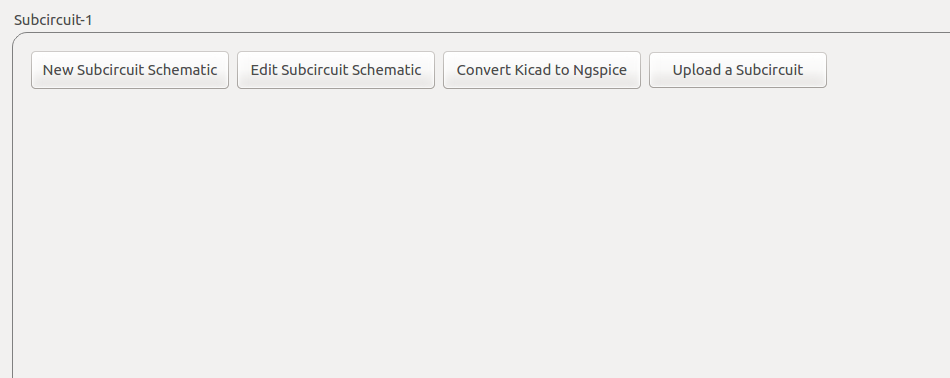
\includegraphics[width =\lgfig]{subcirciut_window.png}
\caption{Subcircuit Window}
\label{subcircuit_mainwin}
\end{figure}


\section{Creating a Subcircuit}
%Let us take an example of Half-adder circuit. To create a new sub circuit select the New Subcircuit Schematic.\figref{halfadder} shows the half-adder circuit. %and \figref{block} shows the block of the sub circuit included in the main circuit.
%\begin{figure}[!htp]
%\centering
%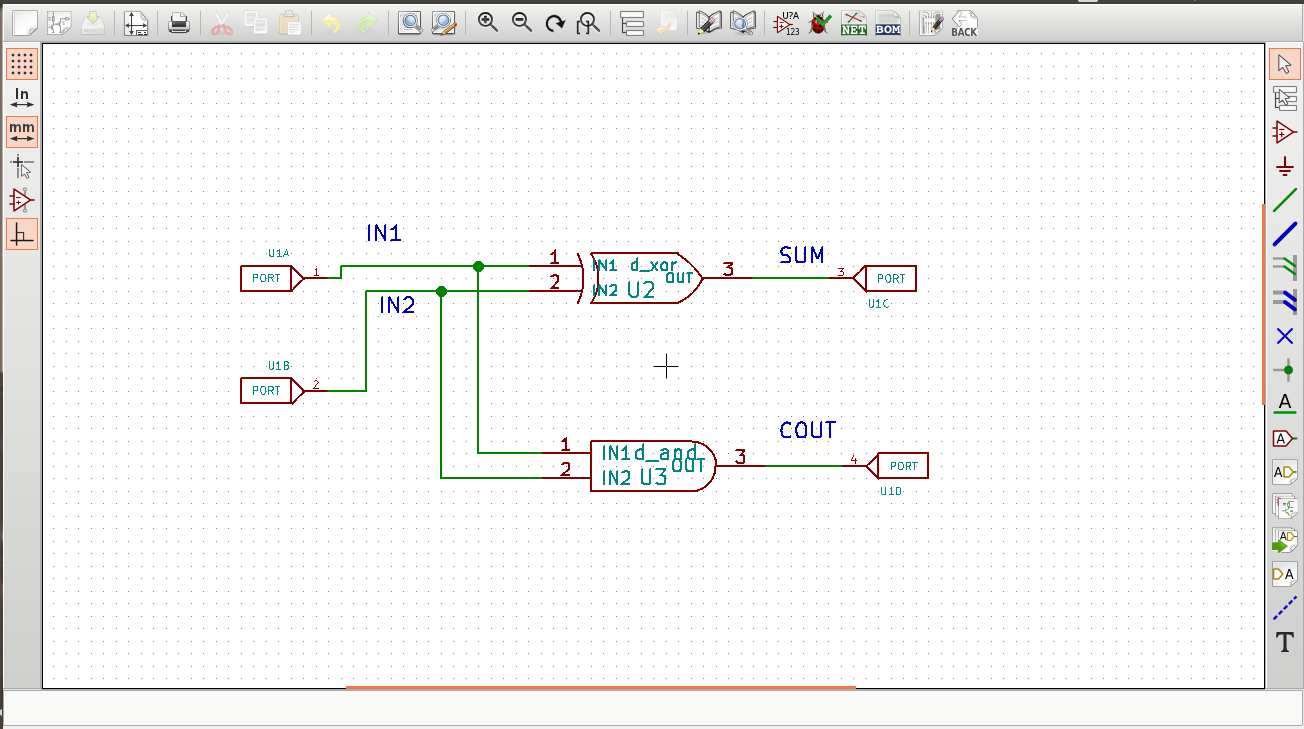
\includegraphics[width = 13cm, height= 7cm]{figures/half_adder.png}
%\caption{Half-Adder Sub-circuit }
%\label{halfadder}
%\end{figure}
%\textit {NOTE: All the input and output of the sub circuits are connected to the port component.}
%\begin{figure}
%\centering
%\includegraphics[width = 8cm, height= 7cm]{figures/halfadderblock.png}
%\caption{Half-Adder Sub-circuit Block }
%\label{block}
%\end{figure}
%After creating the schematic kicad netlist is generated as explained in section and convert kicad to Ngspice where cir.out and .sub files are generated.
%The number of input and output ports of the subcircuit is to matched with number of connections in the main circuit. eSim provides this validation of mapping of the sub circuit ports.
%Also the respective input and output ports can be checked by reading the .sub file.
The steps to create subcircuit are as follows.
\begin{itemize}

\item After opening the Subcircuit tool, click on {\tt New Subcircuit Schematic} button. It will ask the name of the subcircuit. Enter the name of subcircuit (without any spaces) and click {\tt OK} as shown in \figref{newsubcktschematic}.
      


        \begin{figure}[!htp]
            \centering
            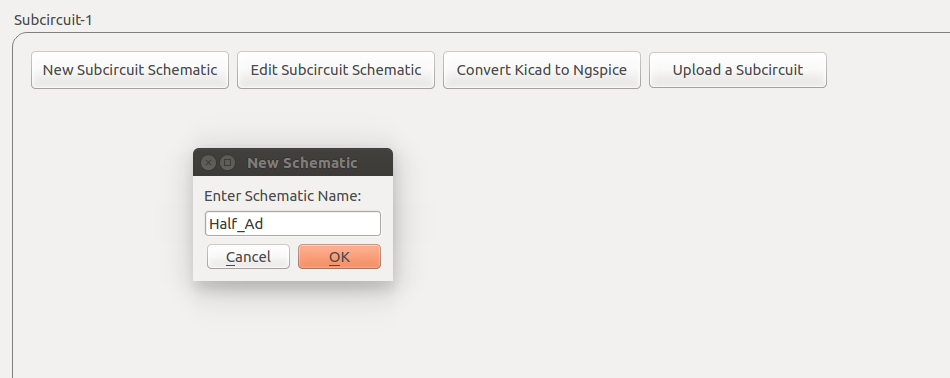
\includegraphics[width =\lgfig]{newsubckt.png}
            \caption{New Sub circuit Window}
            \label{newsubcktschematic}
        \end{figure}

\item After clicking {\tt OK} button it will open KiCad schematic. Draw your circuit which will be later used as a subcircuit. e.g the \figref{createsubcktsch} shows the half adder circuit.
        
        \begin{figure}[!htp]
            \centering
            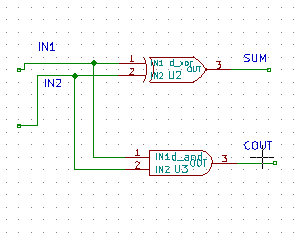
\includegraphics[width =\lgfig]{createsubcktsch.png}
            \caption{Inner circuit of the subcircuit}
            \label{createsubcktsch}
         \end{figure}



\item Once you complete the circuit, assign a PORT to each open node of your circuit which will be used to connect with the main circuit. The port should match with the number of input and output pin. The circuit will look like \figref{halfadder} after adding PORT to it. The PORT component can be found in the eSim\_Miscellaneous library as shown in \figref{port}. Select a different port for each node (input or output), the PORT has 26 such components named alphabetically as Unit A, Unit B to Unit Z, meaning you can create a subcircuit up-to 26 pins(input, output combined).
        
    
        \begin{figure}[!htp]
            \centering
            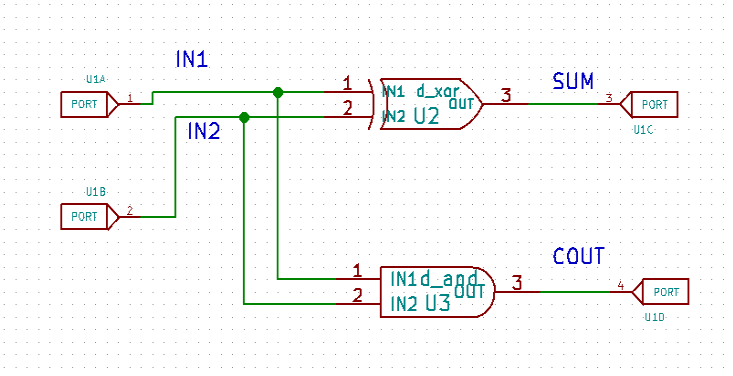
\includegraphics[width =\hgfig]{ha_sub.png}
            \caption{Half-Adder Subcircuit }
            \label{halfadder}
        \end{figure}


        \begin{figure}[!htp]
            \centering
            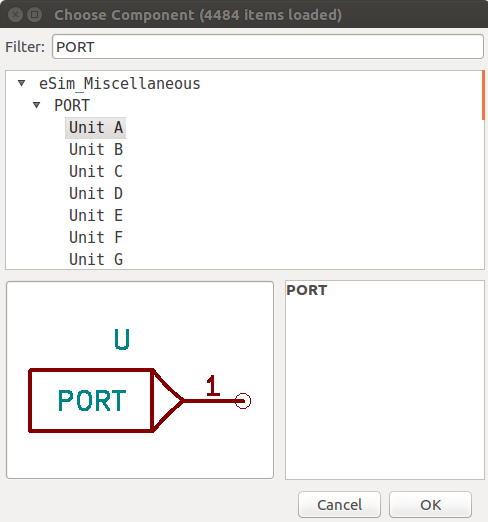
\includegraphics[width =\smfig]{misc_port_list.png}
            \caption{Selection of PORT component}
            \label{port}
        \end{figure}

    \item Next step is to save the schematic and generate KiCad netlist as explained in \chapref{chap5}.

    \item To use this subcircuit in other schematics, create a block in the schematic editor by following steps given below as one should have a symbol corresponding to the newly created subcircuit that can be used in other schematics:
        \begin{enumerate}
            \item Go to library browser of the schematic editor. It is an "open book with a pencil in its middle" icon on the top toolbar.
            \item Select the Current Library as eSim\_Subckt shown in \figref{esimsubckt} 
                \begin{figure}[!htp]
                    \centering
                    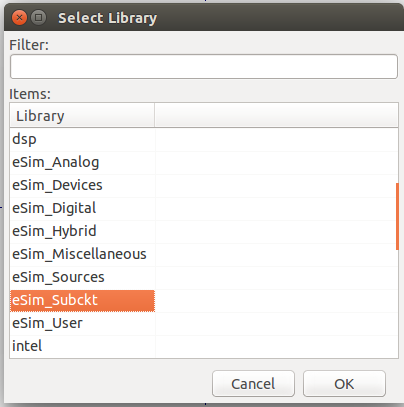
\includegraphics[width =\smfig]{esim-subckt.png}
                    \caption{Selecting Working Library}
                    \label{esimsubckt}
                \end{figure}
            \pagebreak

        \item Click on create a new component from the top toolbar.
        \item Give the same name that was used for creating the new subcircuit's internal diagram, refer \figref{newsubcktschematic}.
        \item Choose designator as \textbf{X}. If any other reference designator other than X is used for \textbf{subcircuit}, your subcircuit will not be recognised during simulation.
        \item Similarly, reference designator are as follows for different types of components. D is for diode, Q is for transistors, J is for FET. The user needs to choose the appropriate reference based on the library in which they wish to add a model. 
            \begin{figure}[!htp]
                \centering         
                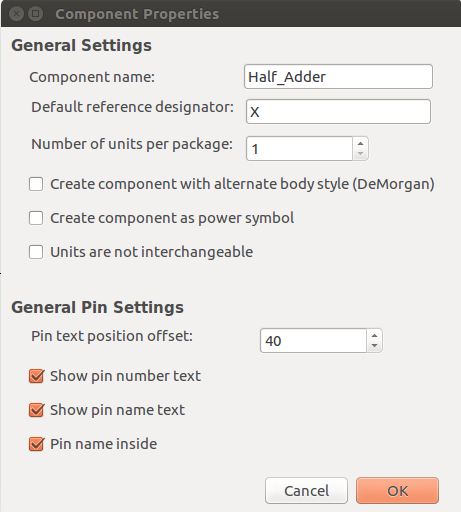
\includegraphics[width =\smfig]{subcktnewcomp.png}
                \caption{Creating New Component}
                \label{subcktnewcomp}
            \end{figure}

        \item Start drawing the subcircuit block by using the drawing tools from the right taskbar. Here we have used \textbf{Add graphic rectangle to component body}. You can start drawing with a point to point click on the editor.
        \item To add pins select {\textbf {Add pins to components}} from the right taskbar. Give the {\tt Pin Name} as {\tt {IN1}} and {\tt{Pin Number as 1}}. The pin number has to match with the {\tt Port name}. Example Port A is mapped to pin 1. Select the {\textbf{ Orientation}} as right or left accordingly. The {\textbf{ Electrical Type}} has to be chosen as {\tt Input} for nodes which will act as Input in the subcircuit you are creating. Similar logic is for output nodes. We would recommend to declare the ports as either Input, Output or Passive.
        
        \item The final block of the subcircuit would look as shown in \figref{block}. Pins should be attached properly. Labels(Names to the PORTs) should be given such that it is intuitive and someone other than you should be able to understand and use that block with least amount of hassle.
        
        \item In order to save this file, press \textbf{Ctrl+S} keys and click \textbf{yes} for confirmation purposes. 
        
        \item Note : A good practice to retain this created subcircuit would be to take a backup of this library. To do that, click on \textbf{File} from the library editor window and select the \textbf{Save Current Library as} option. A location needs to be selected, please select \textbf{eSim-Workspace} as the location for storing this file and give relevant name e.g. \textbf{eSim-Subckt-backup}. Later other users can use this in their circuits.
        
        
                    \begin{figure}[!htp]
                        \centering
                        \includegraphics[width =\smfig]{halfadderblock.png}
                        \caption{Half-Adder Subcircuit Block}
                        \label{block}
                    \end{figure}
\end{enumerate}
        
\subsubsection{Specifying parameters for generating the \textbf{.sub} file }
\begin{enumerate}
\item A \textbf{.sub} file is nothing but textual representation that is passed to the simulator which essentially informs the simulator about the nodes, and behavior of the subcircuit block.
Remember the \figref{halfadder} circuit? It will be saved in a \textbf{.sub} file once we complete this process!
 \item Switch to the eSim main window and click on \textbf{Convert KiCad to Ngspice button} in the \textbf{subcircuit builder tool}. as shown in \figref{subcircuit_mainwin}
 \item You need not assign any values in the transient parameters section. \\
 Assign the values to any voltage or current sources present in your internal circuit, if any. \\
 Add the appropriate device libraries or subcircuit libraries if you have used any Device Models or  Subcircuits, if any. 
 \item Upon successful generation of the subcircuit file, an acknowledgement message will be displayed. To confirm, go to \\
 \large \textit{For Windows OS users} : \\
 \large {C:/FOSSEE/eSim/Library/SubcircuitLibrary if you are using v2.0 and above} \\
 \large C:/FOSSEE/eSim/src/SubcircuitLibrary if you are using versions \textbf{lower than 2.0} \\
 
 \large \textit{For Ubuntu Linux Users} \\
 ../eSim-2.0/Library/SubcircuitLibrary if you are using v2.0 and above \\
 ../eSim-1.1.3/src/SubcircuitLibrary if you are using versions \textbf{lower than 2.0} \\
 And make sure that the .sub file is present under the directory carrying the name of the subcircuit that you specified in step in \figref{newsubcktschematic}.
 
 \end{enumerate}

\end{itemize}

\section{Edit a Subcircuit}
The steps to edit a subcircuit are as follows.

\begin{itemize}
    \item After launching the Subcircuit tool, click on \textbf{Edit Subcircuit Schematic} button. It will open a dialog box where you can select any subcircuit for editing.
    \item After selecting the subcircuit it will open it in the schematic editor, where you can edit the subcircuit.
    \item Next step is to save the schematic and generate the .cir netlist.
    \item If you have edited the number of ports then you have to change the block exaplained in section {Creating a Subcircuit} accordingly.
\end {itemize}
    
{\textbf{Note}}:    
    
\begin{itemize}
\item User can also import or append the schematic of different projects in the current page using the \textit{Append Schematic Sheet} from the \textit{File} menu. This will import(copy) the schematic that user has defined to the current schematic editor page.
\item  User can also import the model in the part library editor page using the option \textit{Import Component} from the top toolbar.
\end{itemize}

\section{Upload subcircuit}
\begin{itemize}
    \item Using this feature, one can import an existing subcircuit file into eSim environment. You necessarily need not create the schematic for this.
    \item Download the required subcircuit's .sub file from many online resources/repositories. 
    \item Upload this file using the upload subcircuit feature.
    \item Upon uploading following checks will be made, and only and only if the checks are satisfied, the file will be uploaded. The checks are as following : \\
    1. The uploaded file should have the extension \textbf{.sub} \\
    2. The name of the file, say for example is \textbf{omega.sub}, then the content of the file must start with \textbf{.subckt omega} and end with \textbf{.ends omega}. \\
    Any line that starts with asterisk sign(*) is considered as a comment in these types of files. Hence, the file technically starts with \textbf{.subckt}.
    \item If above conditions are satisfied, then the file will be automatically placed in a folder that carries the same name as that of the .sub file will be created in ../SubcircuitLibrary/ directory.
    \item Once above steps are verified, proceed to create a block as shown in \figref{block} and name should be same as that of the corresponding .sub file uploaded earlier. Pins of this block should match the number of pins stated in the .sub file. \\
    NOTE: ONLY AND ONLY THE OUTER BLOCK NEEDS TO BE CREATED. INTERNAL CIRCUIT IS NOT REQUIRED IF YOU ARE USING THE UPLOAD FEATURE.
    
\end{itemize}
